\chapter*{Supplementary Information}

\section*{Data sets}

% \begin{table}[h]
%   \begin{threeparttable}
%     \caption{Public Data sets Analyzed}
%     \begin{tabularx}{@{}llll@{}}
%       \toprule
%       Data set & Figure &  Accession & Reference \\
%       \midrule % column names
% 
%       Lung Fibroblast Hi-C, \gls{hESC} Hi-C & GSE43070 & &\bibentry{jin2013} \\
%       COSMIC Lung Cancer Mutations & &  &\bibentry{forbes2009} \\
%       H1 \gls{hESC} Gene Signatures & GSE54186 & &\bibentry{kim2014} \\
%       IMR90 Gene Signatures & GSE2672 & &\bibentry{kim2005} \\
%       \bottomrule
%     \end{tabular}
%     \begin{tablenotes}
%       All data sets were obtained as of December 2014.
%     \end{tablenotes}
%   \end{threeparttable}
% \end{table}

\section*{Gene Expression Histograms}

\begin{figure}
  \centering

  \begin{subfigure}[b]{0.45\textwidth}
    \centering
    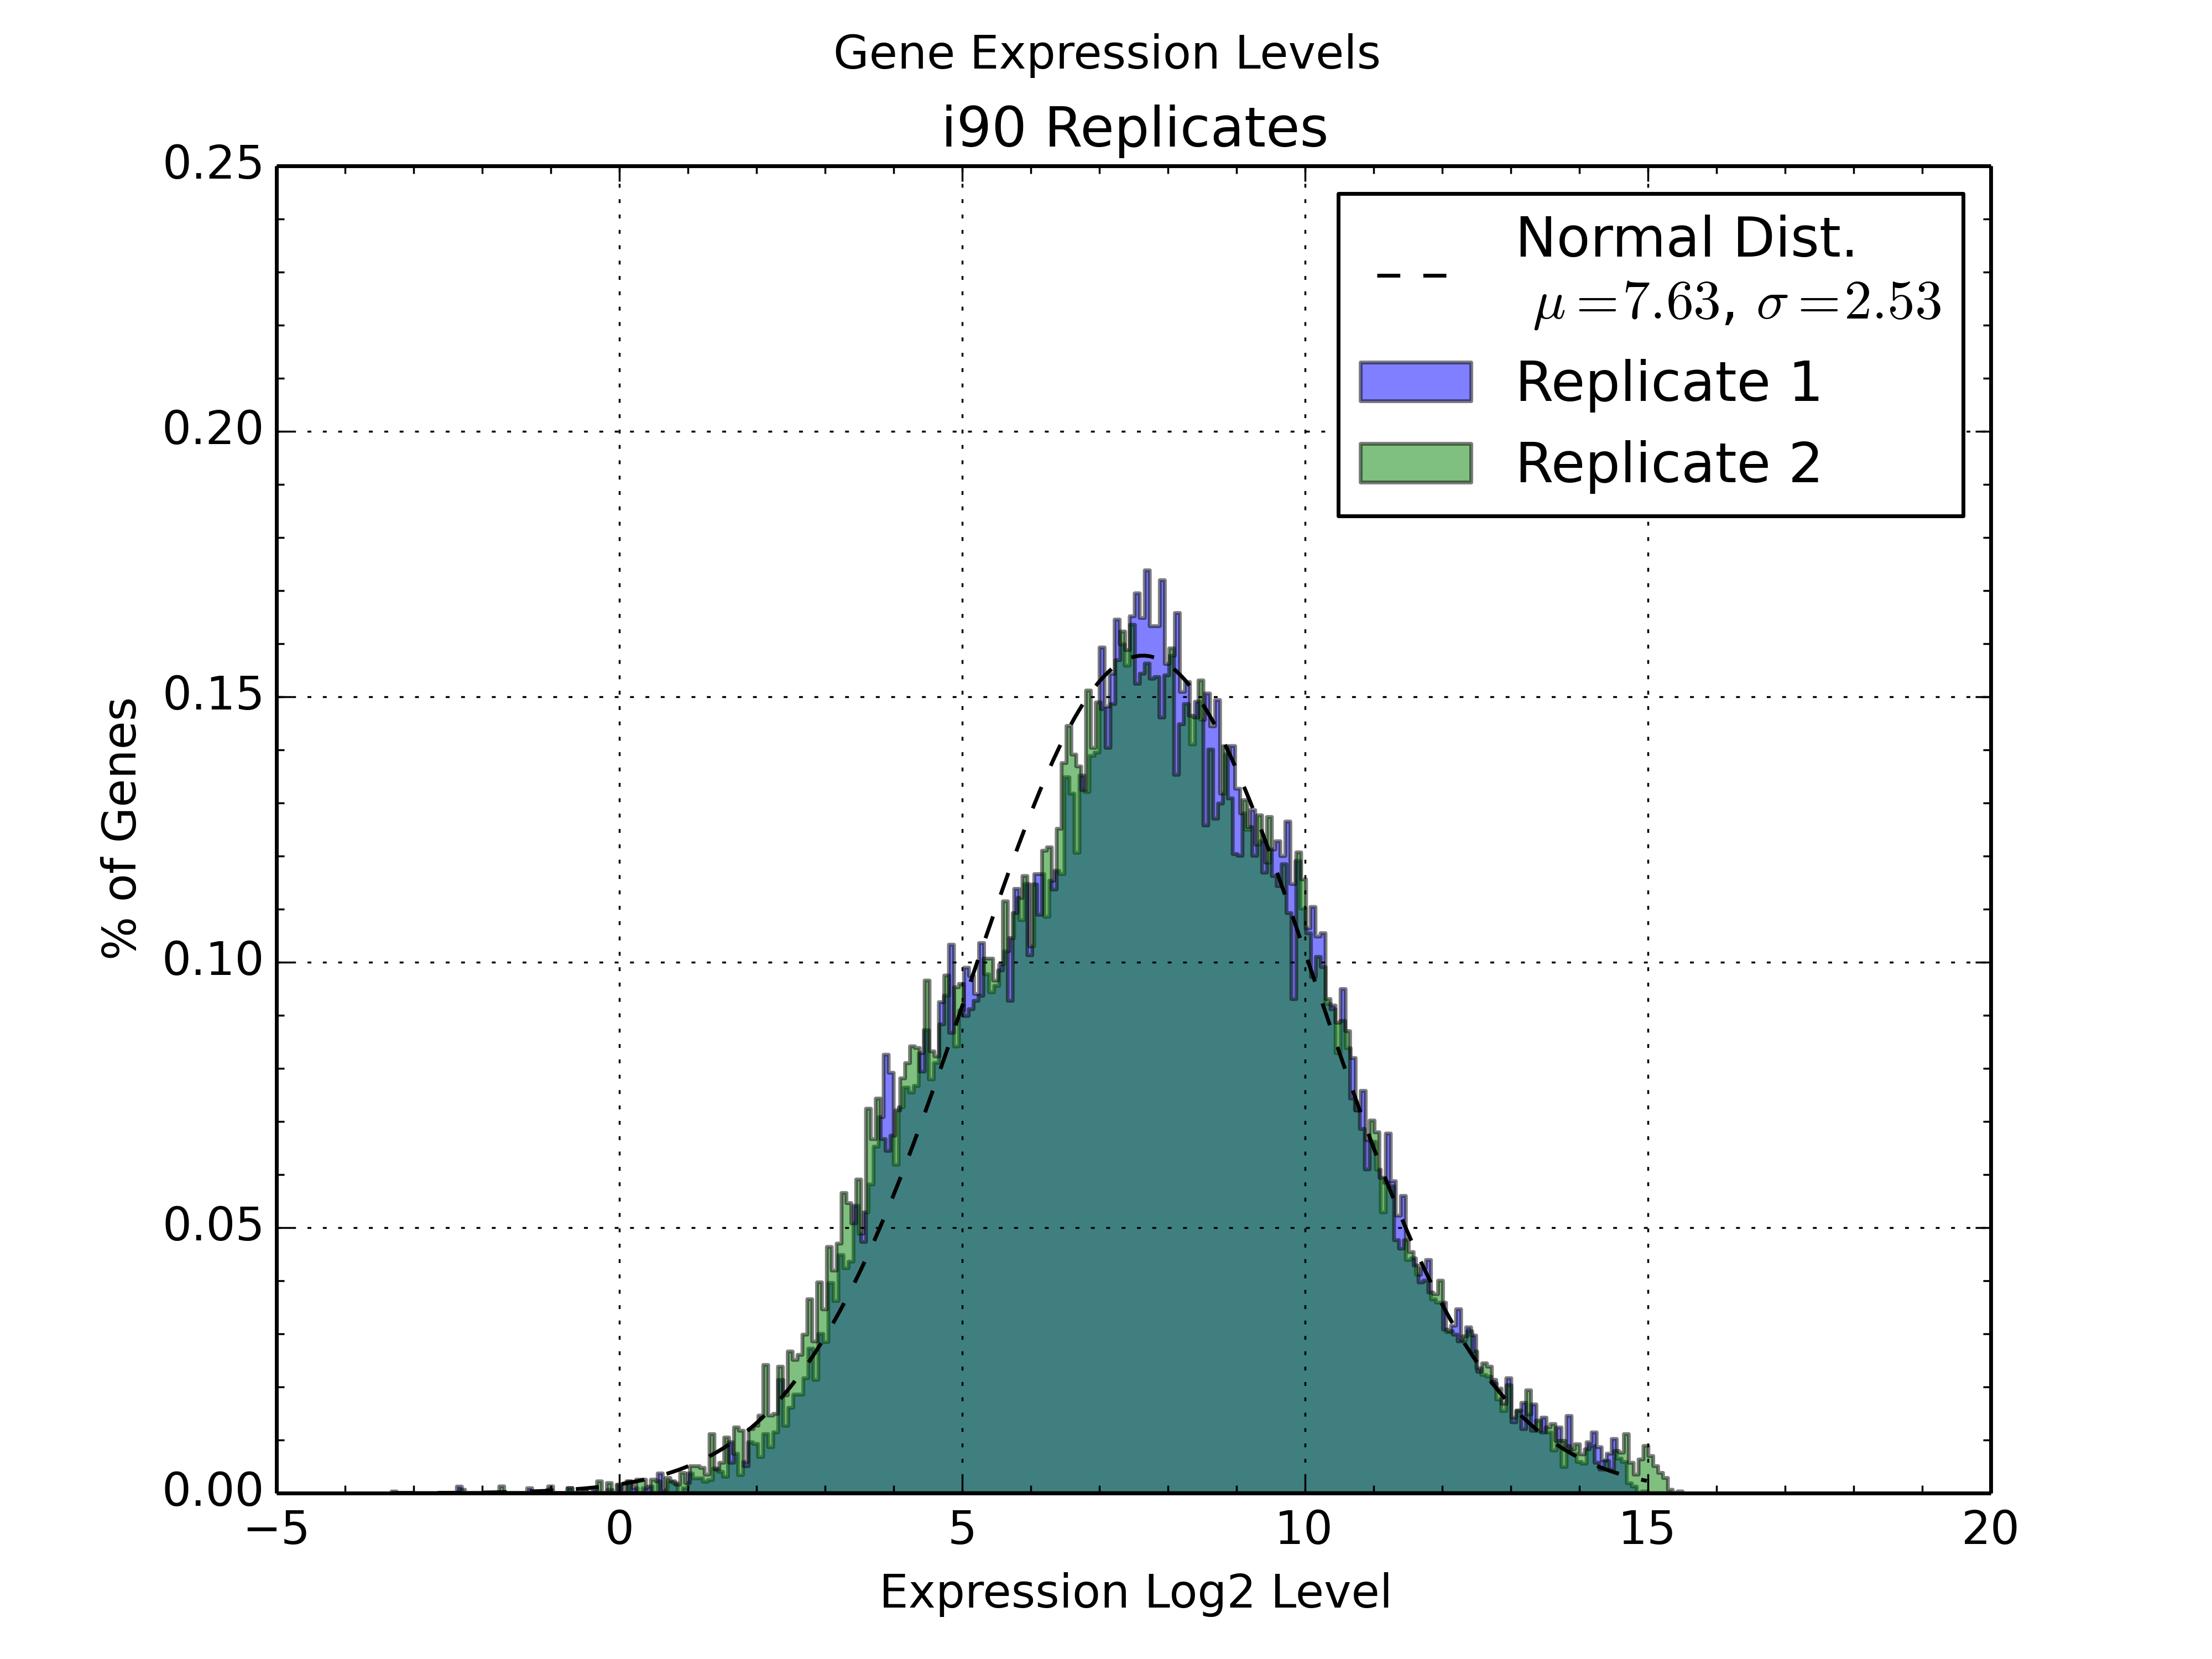
\includegraphics[width=\textwidth]{./fig/supplementary/i90-expression-levels.png}\label{fig:190Expression}
  \end{subfigure}

  \hfill

  \begin{subfigure}[b]{0.45\textwidth}
    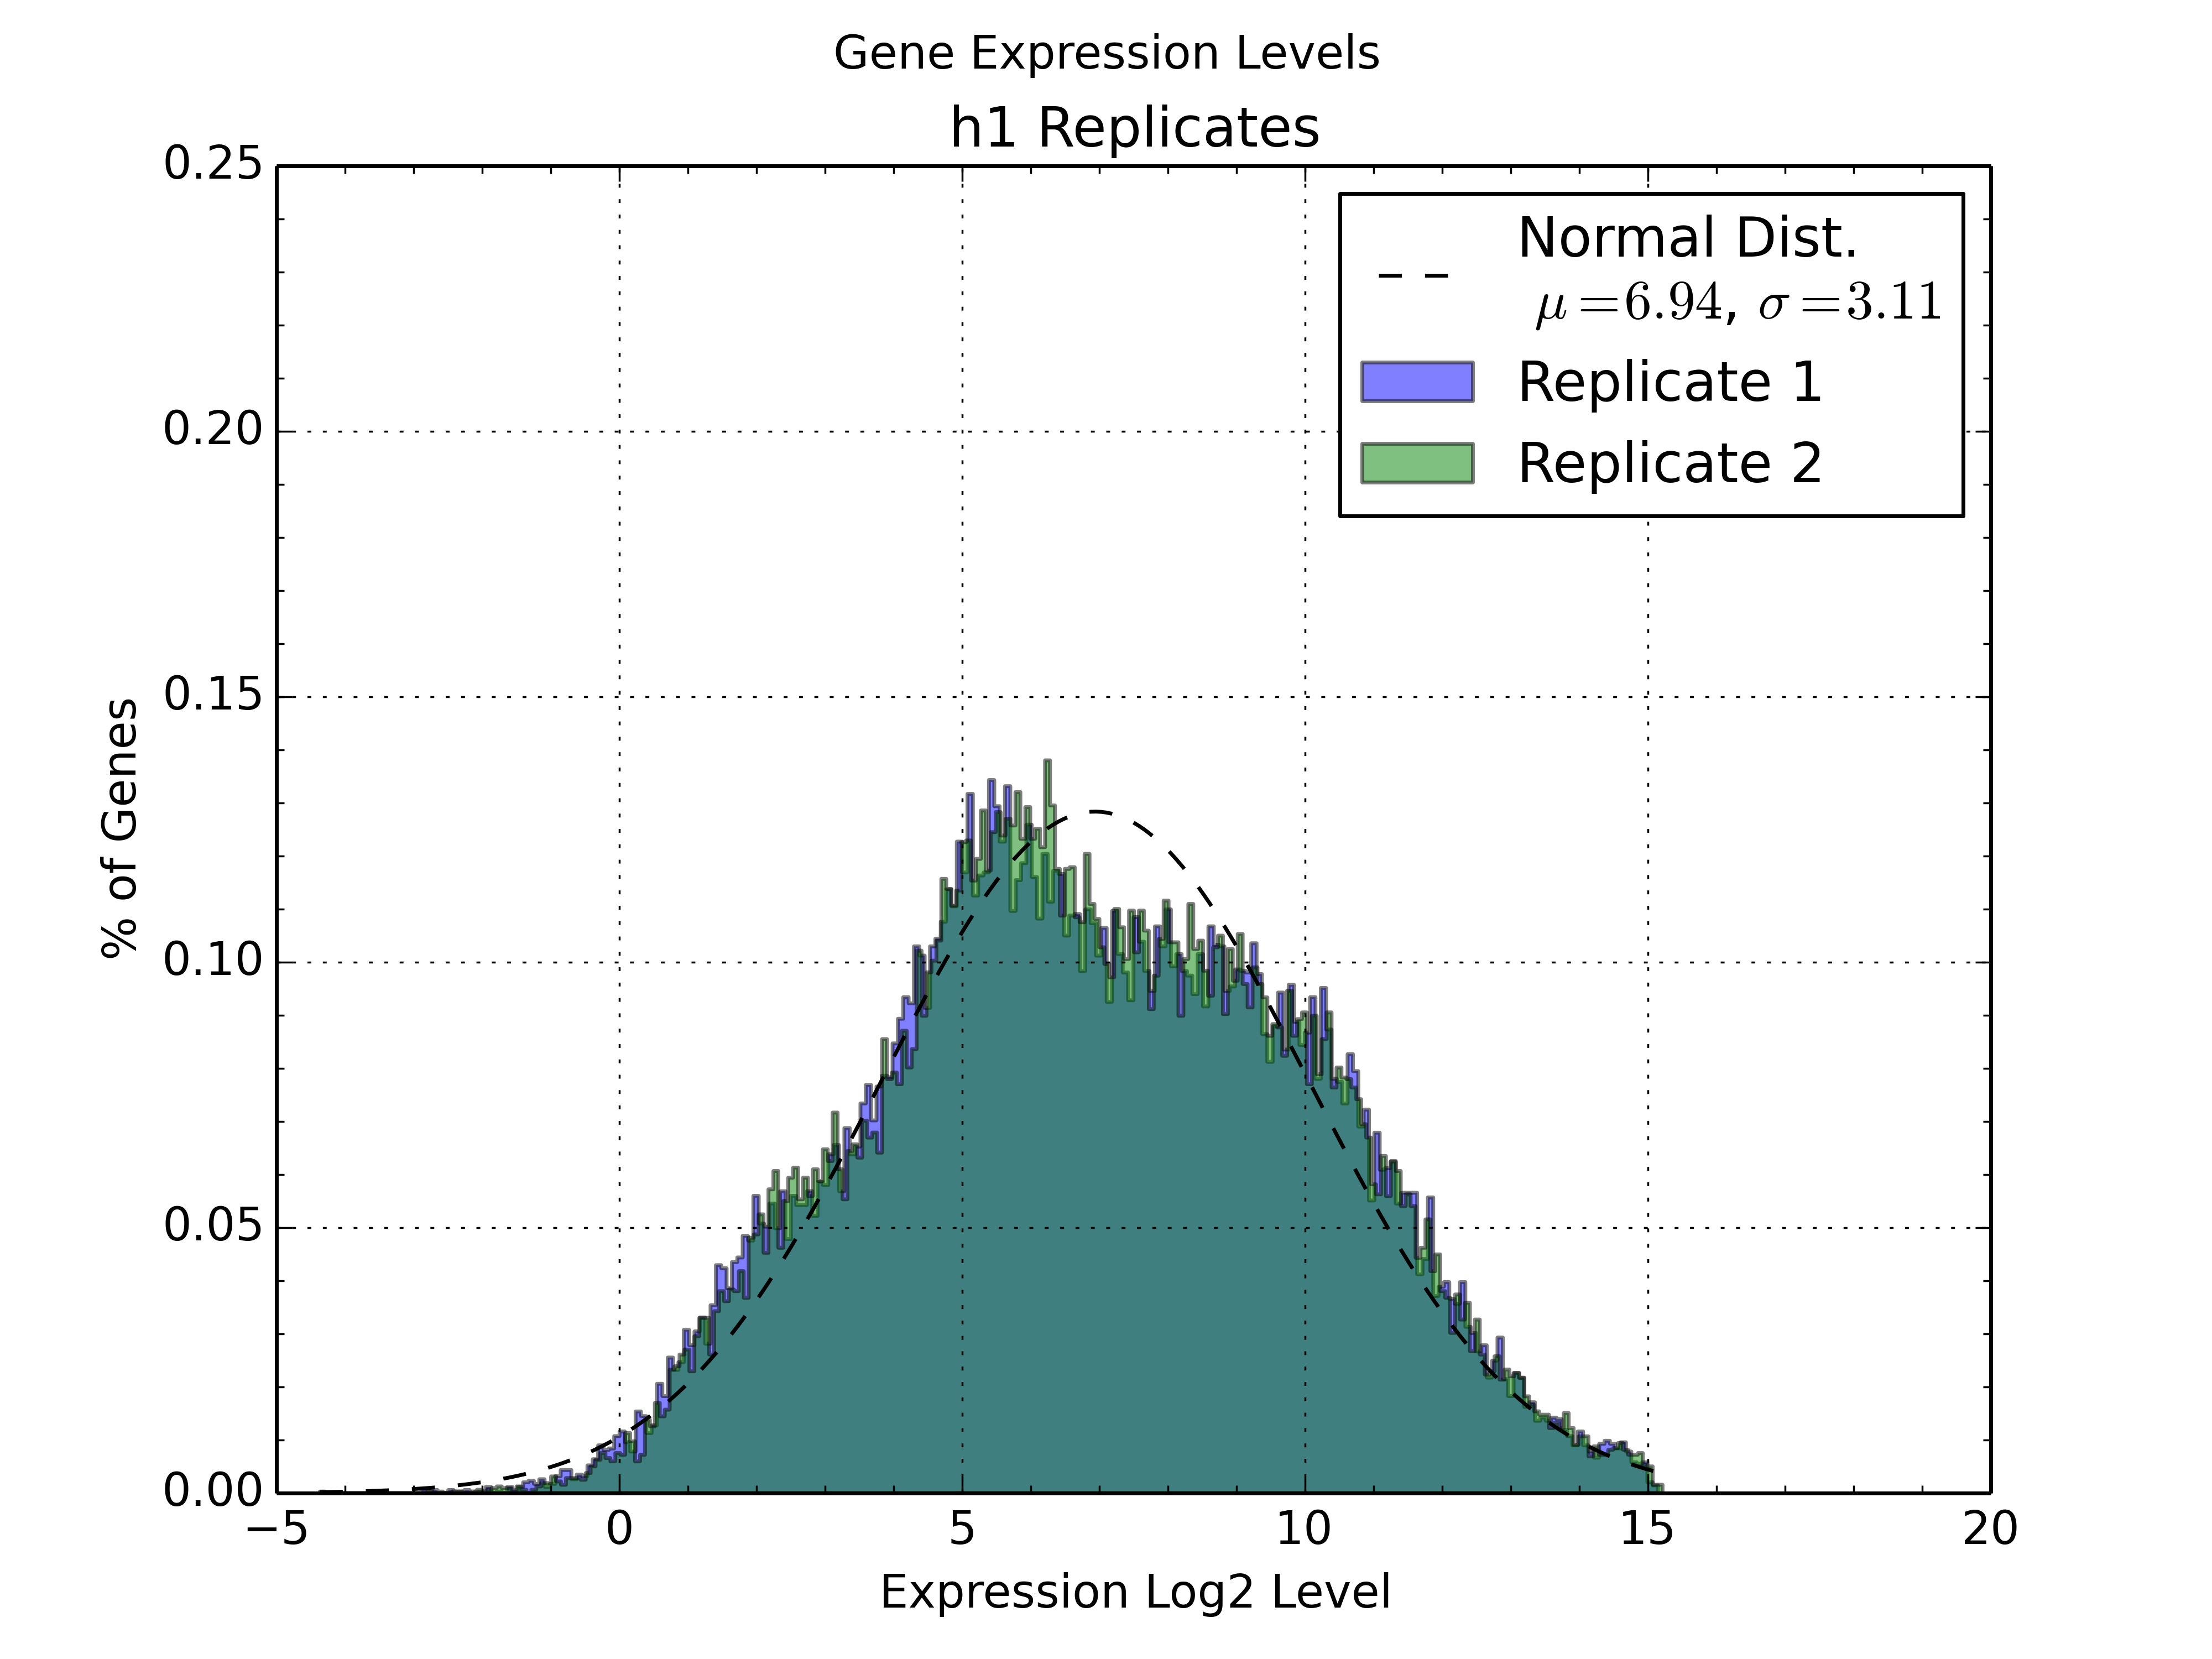
\includegraphics[width=\textwidth]{./fig/supplementary/h1-expression-levels.png}\label{fig:h1expression}
  \end{subfigure}

  \quad

  \begin{subfigure}[b]{0.45\textwidth}
    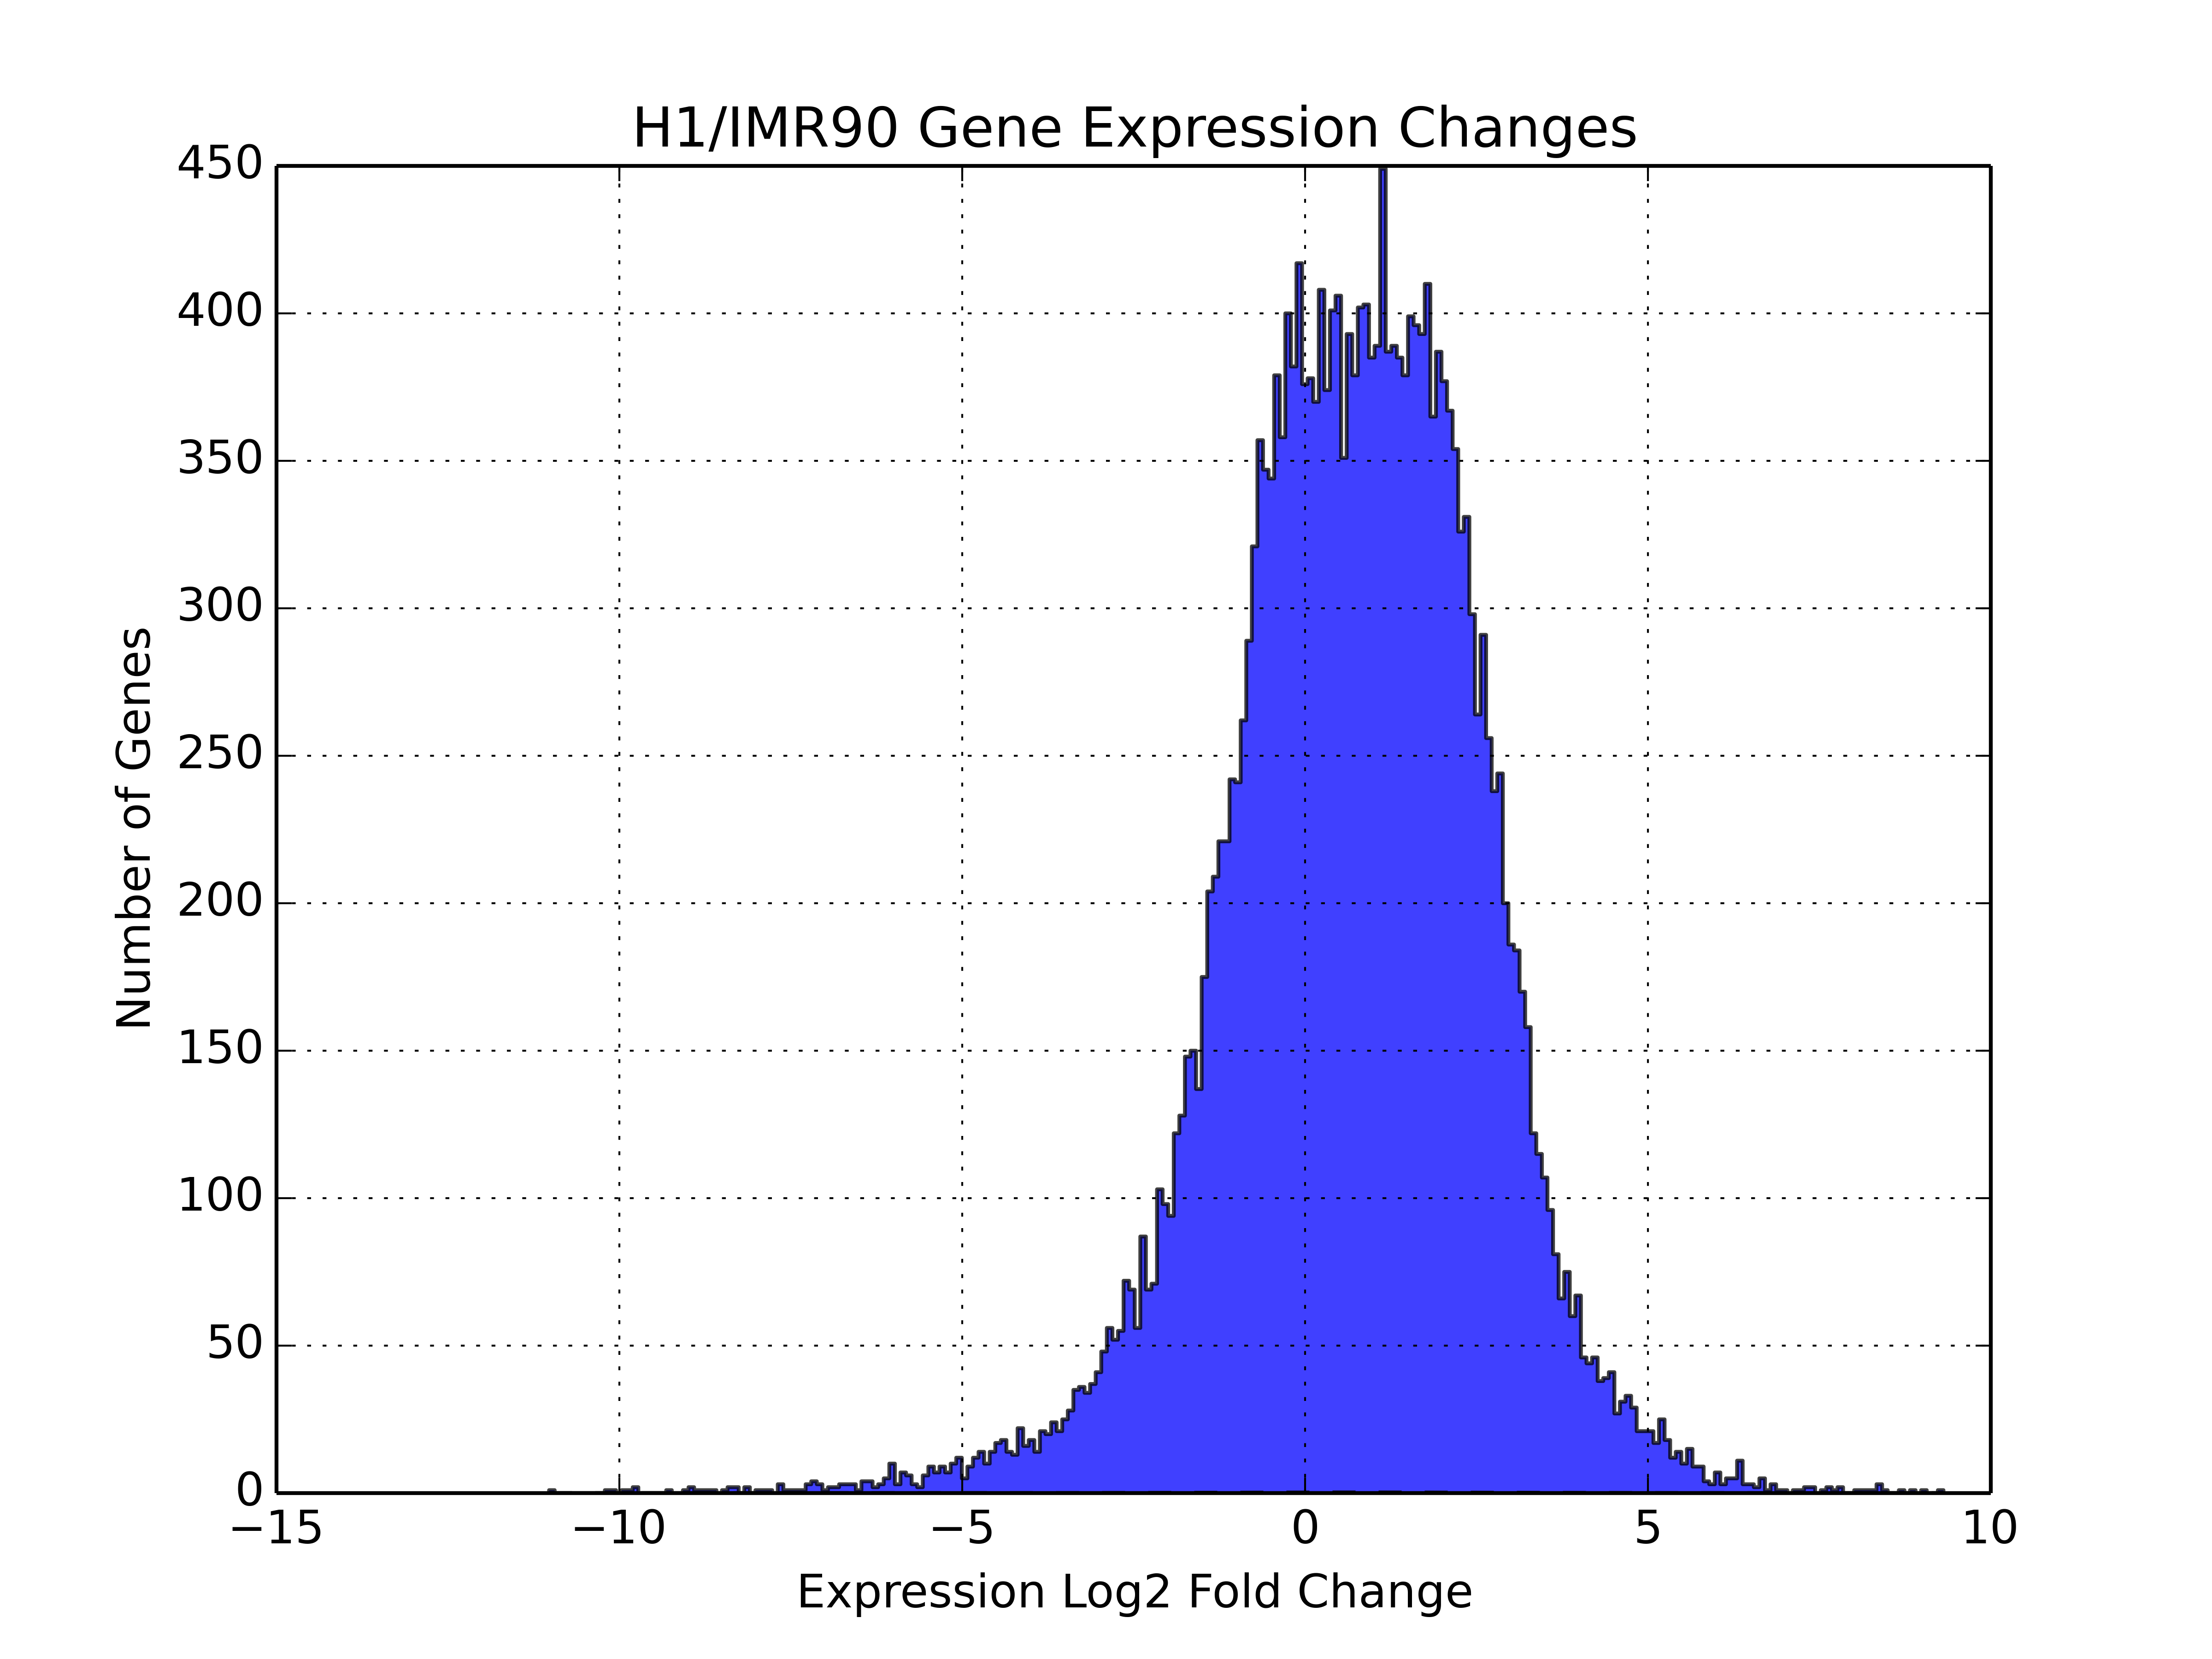
\includegraphics[width=\textwidth]{./fig/supplementary/expressionDelta.png}\label{fig:i90h1expression}
  \end{subfigure}
\end{figure}

\section*{Correlations between Principal Components}

We calculated the pearson correlation coefficients between the first principle components each dataset.

% data from  pca/correlations/*.csv
\begin{table}[h]
  \centering
  \caption{Correlation of PC1 between all experimental replicates}\label{table:PC1Correlations}
  \begin{tabularx}{\textwidth}{@{}cccccccc@{}}
    \toprule
    \multicolumn{6}{l}{IMR90} & \multicolumn{2}{l}{hESC} \\
    \midrule
    \textbf{R1} & 0.981       & 0.972       & 0.983       & 0.983       & 0.977       & 0.656       & 0.658 \\
    0.981       & \textbf{R2} & 0.985       & 0.982       & 0.976       & 0.974       & 0.654       & 0.652 \\
    0.972       & 0.985       & \textbf{R3} & 0.982       & 0.977       & 0.980       & 0.634       & 0.629 \\
    0.983       & 0.982       & 0.982       & \textbf{R4} & 0.986       & 0.982       & 0.655       & 0.655 \\
    0.983       & 0.976       & 0.977       & 0.986       & \textbf{R5} & 0.98        & 0.633       & 0.633 \\
    0.977       & 0.974       & 0.980       & 0.982       & 0.985       & \textbf{R6} & 0.610       & 0.607 \\
    0.656       & 0.654       & 0.634       & 0.655       & 0.633       & 0.610       & \textbf{R1} & 0.973  \\
    0.658       & 0.652       & 0.629       & 0.655       & 0.633       & 0.607       & 0.973       & \textbf{R2}    \\
    \bottomrule
  \end{tabularx}
\end{table}

We also examined the scree plots of each \gls{PC} by experiment and replicate.  The plot for hESC R1 is included for reference.

\begin{figure}
  \centering

  \begin{subfigure}[b]{0.45\textwidth}
    \centering
    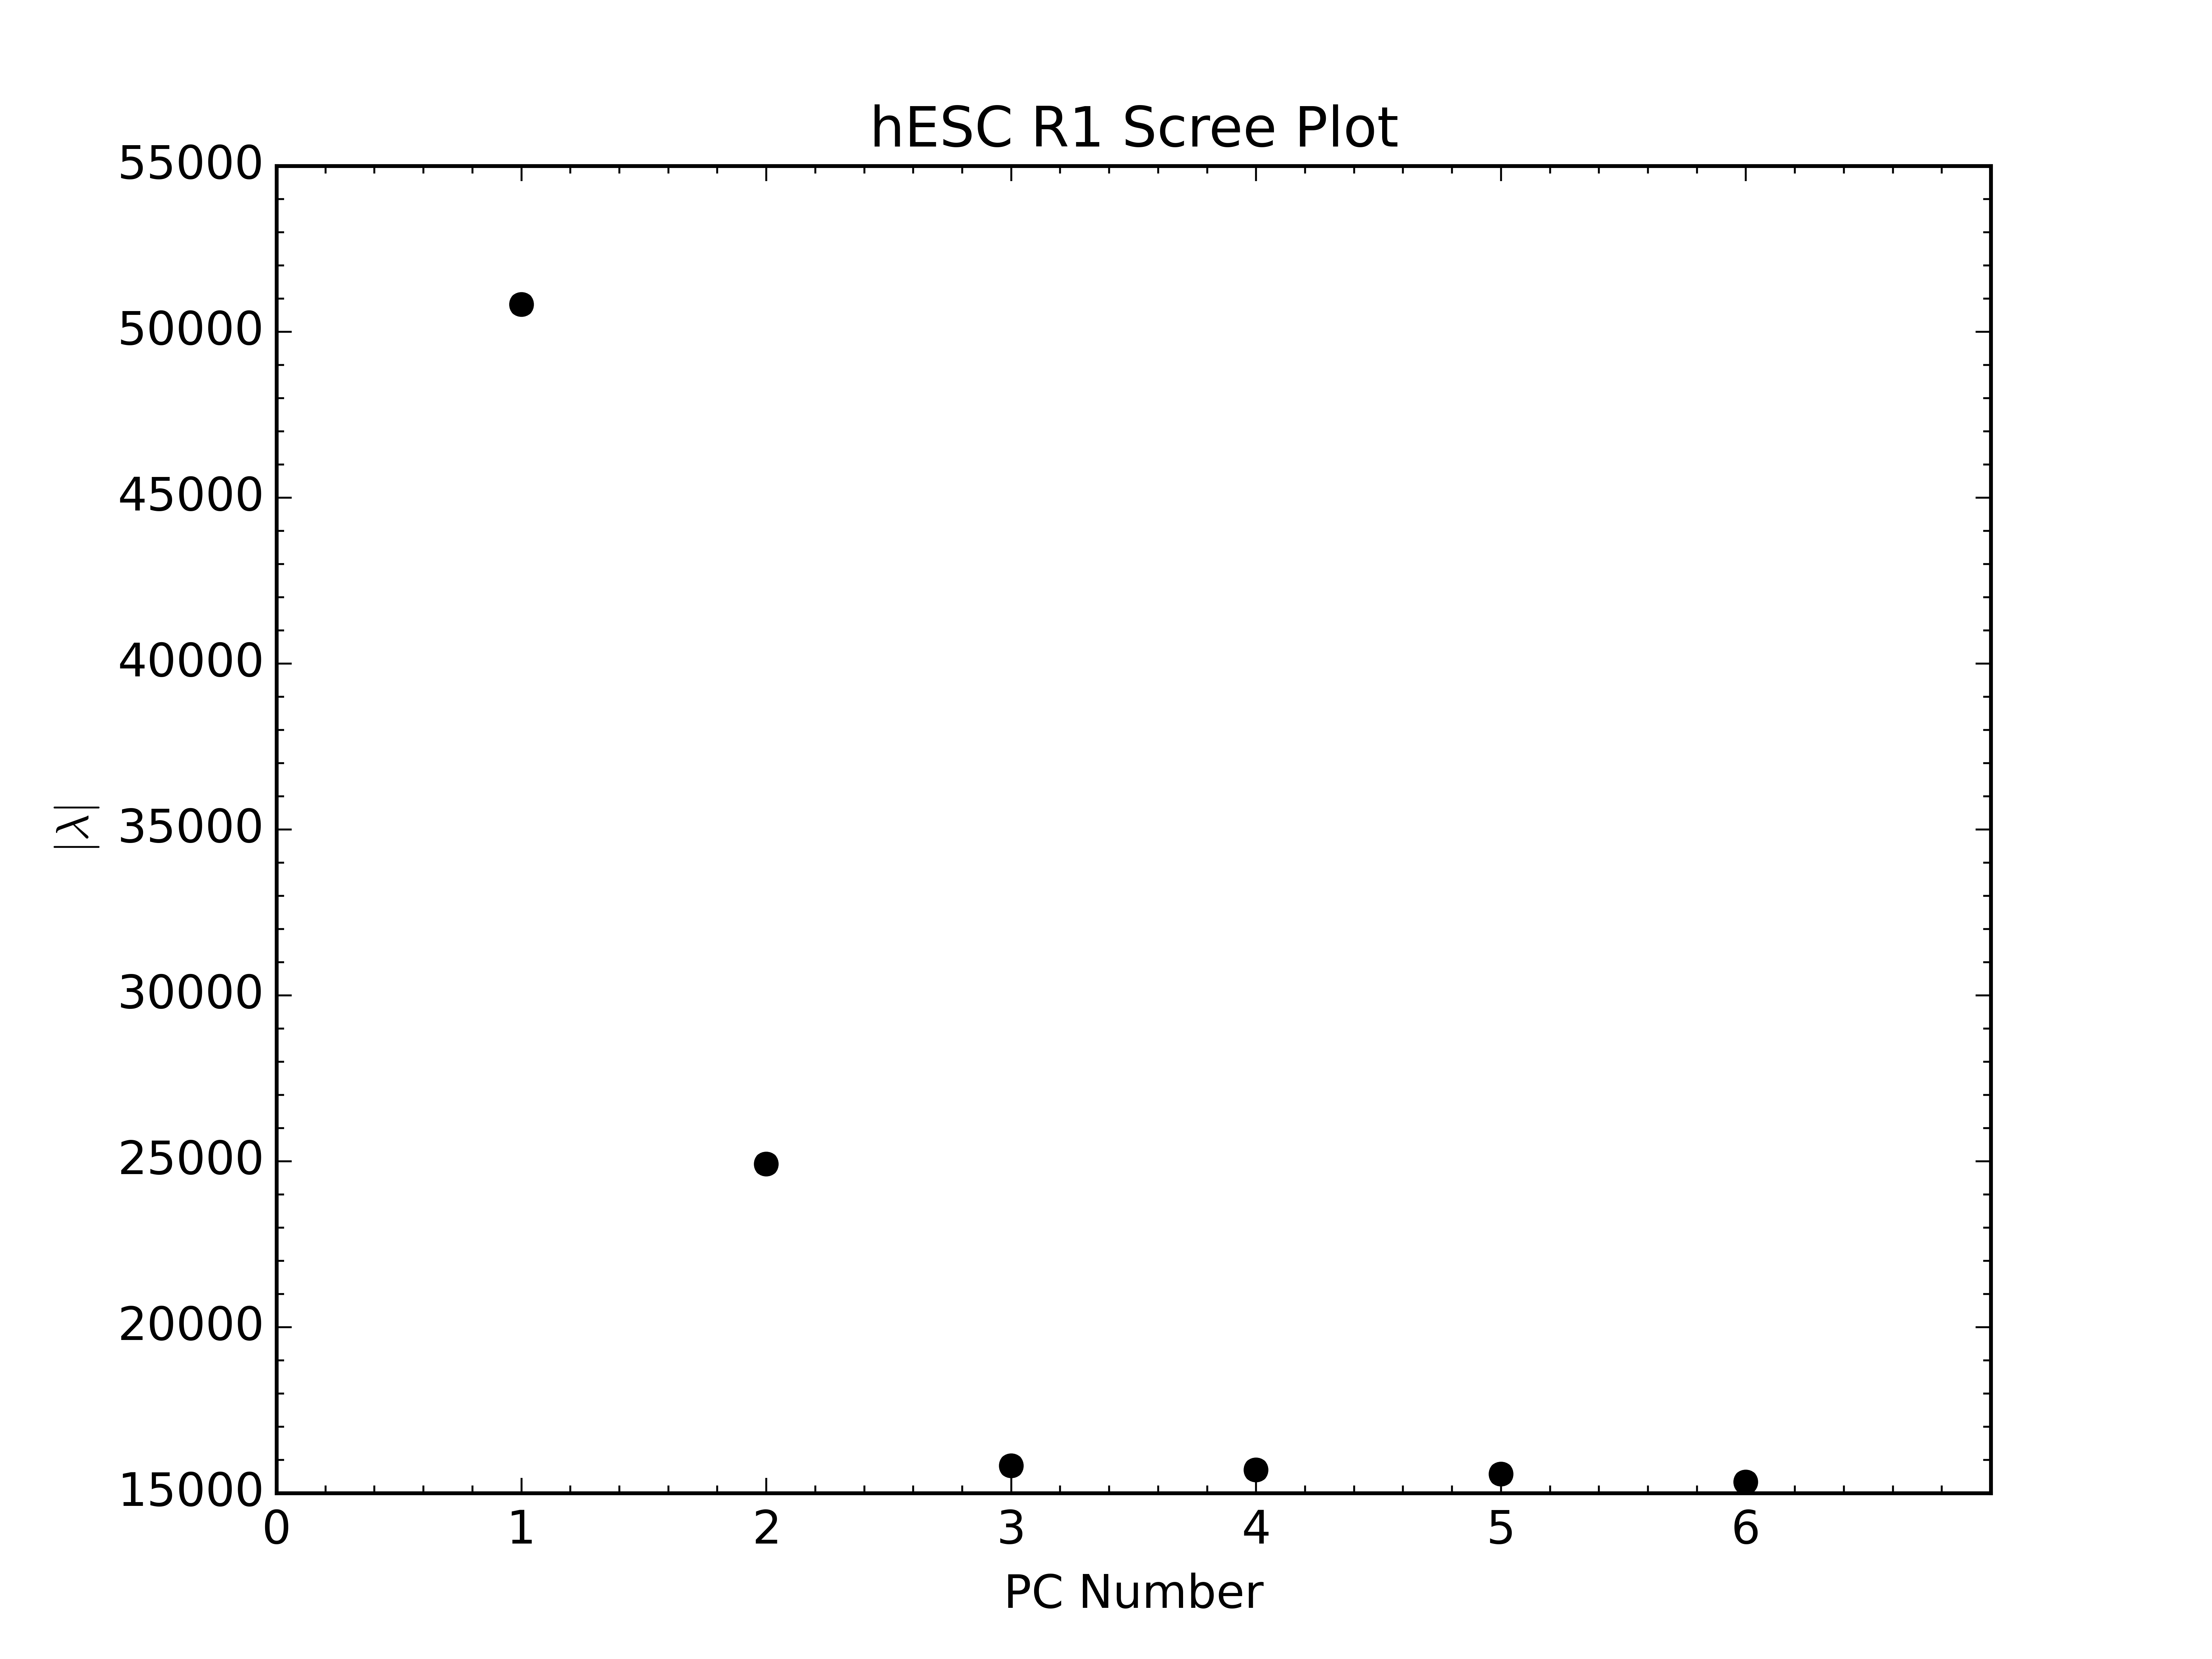
\includegraphics[width=\textwidth]{./fig/supplementary/hESC-R1-scree.png}\label{fig:hESCScree}
  \end{subfigure}

\end{figure}
